\documentclass[../paper.tex]{subfiles}

\begin{document}
  \subsection{Technology Stack}

  The goal of this project in terms of the implementation was to
  build a web application that is easily embeddable into a mobile application.
  For this reason we decided on going for a lean front end without too many
  unnecessary dependencies to keep it responsive. Among the key dependencies that
  are necessary is D3.js, a JavaScript library for manipulating documents based
  on data \cite{d3}. D3 fits the requirements of simple interoperability between
  data and visualisation by manipulating the DOM perfectly.

  Given that the
  visualisation is built around a semantic knowledge graph, a graph database is
  a necessity.

  For the implementation, an instance of  GraphDB \cite{graphdb}, a proprietary graph
  database developed by Ontotext, was used. It offers multiple APIs for querying the database,
  including RDF4J and SPARQL, among other things. The multiple APIs offered by
  GraphDB allowed us to use a vendor-agnostic JavaScript framework for
  creating SPARQL queries. As the overall goal was simplicity and reusability,
  SPARQL was used querying data, since it is widely used
  in the semantic community and well adopted. This makes the application work with
  basically any graph database, which supports data fetching with SPARQL.

  A simple use case would be a user starting the application, which initialises
  the D3 front end web application, which in turn queries data from the database
  to visualise the consent page as shown in \cref{fig:prototype}.

  \subsection{Architecture}

  Shown in \cref{fig:architecture} is an overview of the technical architecture
  for the implementation of the data visualisation.

  \begin{figure}
    \centering
    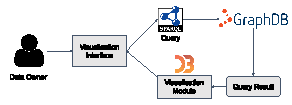
\includegraphics[width=\linewidth]{architecture.pdf}
    \caption{Technical Architecture}
    \label{fig:architecture}
  \end{figure}

  On the left side of \cref{fig:architecture} we see the application user, i.e.
  the data owner. The data owner interacts only with the front end part of the
  application, which we call the “Visualisation Interface”.

  On first load or whenever the user interacts with the interface in such a way
  that the underlying data needs to be updated, we send a SPARQL query to the
  GraphDB database. Once the result of this query is retrieved, it is passed to
  the “Visualisation Module”. This module processes the data depending on
  whether it will be displayed in the overview visualisation or the detailed
  time series visualisation and produces the corresponding visualisation
  using D3.js accordingly.

  Depending on the query, we get a lot of data in return, as the database
  will return a value for each data-package, that was sent. The so called
  "Visualisation Module" groups those together, creating a single visible
  node for each category of data. These categories are predefined in the
  ontology and represent thing like coordinates, longitude and latitude, or
  fuel consumption. The module then creates connections between the data packages
  and the third party companies receiving them. One can think of this module
  as the pure front end of the application.

  After the visualisation is created for the received data, the “Visualisation Module”
  updates the currently displayed graph. This can easily be done with D3.js, since
  it creates a graph context, which can be modified directly. Therefore,
  we can add or remove nodes from the graph and directly update the visualisation
  upon the receiving a users input.

\end{document}
